\section{Lesson learned}
In this section I have described all the models I have created over time.
From each model I learned something and realized what I could improve.
The models are listed from first to second to last to show the learning journey.

\subsection{First model: IMDb dataset}
The first model I created was with BERT, without any framework I simply followed the official Tensorflow tutorial.
I trained this model the IMDb dataset.
This model was purely for educational purposes, once trained the model the only work that actually there was to do was a little fine tuning.
But honestly, I used this model only as an approach to get into the world of BERT, in fact I followed the tutorial of Tensorflow itself to get to this result.
For a thesis work I wanted to do something of my own, and not using code and tutorial that it can already find on the net, so I tried something different.
After several searches I came across Ktrain.

\subsubsection{Lesson learned}
I learned how to configure a model with the optimizer, loss and metric.

\textbf{What is optimizer?}\\
Optimizers are used for improving speed and performance for training a specific model \cite{noauthor_tensorflow_nodate}. 
For my model I chose Adam optimizer. Adam optimization is a stochastic gradient descent method that is based on adaptive estimation of first order and second-order moments \cite{noauthor_tfkerasoptimizersadam_nodate}.

\textbf{What is loss?}\\
 We use a loss function to determine how far the predicted values deviate from the actual values in the training data. We change the model weights to make the loss minimum, and that is what training is all about \cite{patnaik_loss_2018}.
 
\textbf{What is metric?}\\Calculates how often predictions matches integer labels \cite{noauthor_tfkerasmetricssparsecategoricalaccuracy_nodate}.

\subsection{Second model: Ktrain - Hotel dataset}
To be able to do something of my own I thought to work also on the dataset, so with Ktrain I did not use the IMDB dataset, but I opted for the Hotel Reviews dataset.

\subsubsection{Hotel Review Dataset}
\paragraph*{Dataframe structure}
The CSV file contains 17 columns, this means that one customer rating contains 17 attributes. In Table~\ref{tab:Dataframe structure} all attributes are explained in detail:

\begin{longtable}[ c ]{| m{5cm} | m{8cm}|}
\hline
\multicolumn{2}{|c|}{\textbf{Dataframe structure}}                                                                                                         \\ \hline
\endfirsthead
%
\multicolumn{2}{c}%
{{\bfseries  Table \thetable\ continued from previous page}} \\
\hline
\multicolumn{2}{|c|}{\textbf{Dataframe structure}}                                                                                                         \\ \hline
\endhead
%
\textbf{Hotel\_Address  }                     & Hotel address.                                                                                  \\ \hline
\textbf{Review\_Date}                         & Date on which the customer left his comment.                                          \\ \hline
\textbf{Average\_Score}                       & Average rating. Calculation by all comments of the last year.              \\ \hline
\textbf{Hotel\_Name}                          & Hotel name.                                                                                     \\ \hline
\textbf{Reviewer\_Nationality}                & Client nationality.                                                                             \\ \hline
\textbf{Negative\_Review}                     & Negative review of the customer. If there is no negative review, it says: "No Negative". \\ \hline
\textbf{ReviewTotalNegativeWord Counts}        & Number of words in the negative review.                                                        \\ \hline
\textbf{Positive\_Review}                     & Positive review of the customer. If there is no positive review, it says: "No Positive". \\ \hline
\textbf{ReviewTotalPositiveWord Counts}        & Number of words in the positive review.                                                        \\ \hline
\textbf{Reviewer\_Score}                      & Score Rating.                                                                                \\ \hline
\textbf{TotalNumberofReviews ReviewerHasGiven} & Total number of reviews left by the customer.                                  \\ \hline
\textbf{TotalNumberof\_Reviews}               & Number of reviews of the hotel.                                                                   \\ \hline
\textbf{Tags}                                 & Tags left by the customer for the review.                                                 \\ \hline
\textbf{dayssincereview}                      & Number of days between the evaluation date and creation of the \gls{dataset}.                              \\ \hline
\textbf{AdditionalNumberof \_Scoring} & The number of reviews of the customer, which consist only of a score rating and do not include a comment. \\ \hline
\textbf{lat}                                  & Latitude of the location of the hotel.                                                                 \\ \hline
\textbf{lng}                                  & Longitude of the location of the hotel.                                                                  \\ \hline
\caption{Dataframe structure}
\label{tab:Dataframe structure}\\
\end{longtable}

\subsubsection{Process the data}
To do this first I worked on the dataset so:
\begin{itemize}
    \item cleaned up the columns I did not need,
    \item divided the dataset in positive and negative thanks to the score table, so for a value below 7 is negative and above 7 is positive,
    \item resample so that there are the same number of reviews for positive and negative.
\end{itemize}

Ktrain provides me with a lot of useful features for my purpose.
The first Ktrain function I used is text.texts\_from\_df.
As it is written in the documentation \cite{noauthor_amaiyaktrain_nodate}, this function allows me to:

“Loads text data from Pandas dataframe file. Class labels are assumed to be one of the following formats:
\begin{itemize}
    \item one-hot-encoded or multi-hot-encoded arrays representing classes
    \item labels are in a single column of string or integer values representing class labels
    \item labels are a single column of numerical values for text regression.”
\end{itemize}
The advantage is that I do not have to do every single preprocessing step manually, and all the steps are followed by the library itself.

Mine is case number two, in fact my dataframe in Figure~\ref{fig:fig_24}, is composed as follows:
\begin{figure}[ht!]
\centering
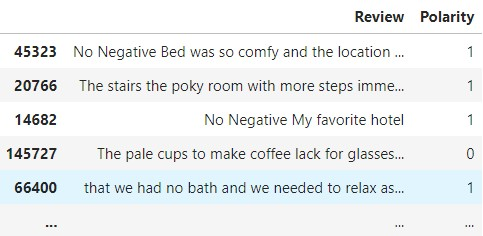
\includegraphics[width=0.65\textwidth]{images/dataframe.jpg}
\caption{My resample dataframe}
\label{fig:fig_24}
\end{figure}
\FloatBarrier

In images below are shown the function from the documentation~\ref{fig:fig_22} and the code function I used:
\begin{figure}[ht!]
\centering
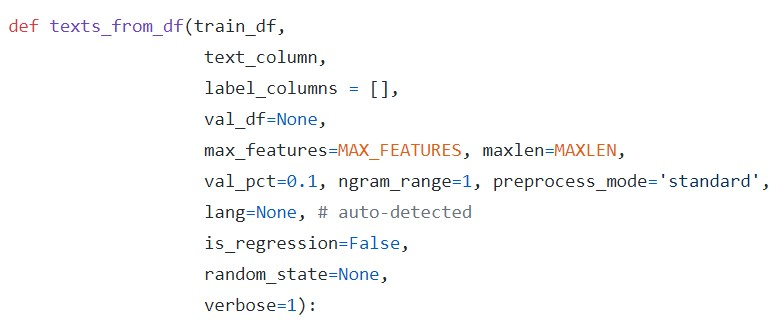
\includegraphics[width=0.75\textwidth]{images/textdf.jpg}
\caption{Ktrain text function from documentation}
\label{fig:fig_22}
\end{figure}
\FloatBarrier
The function will take as feature the column "Review" and as target "Polarity", it will also automatically download an already pretrained DistilBERT model with its vocabulary.
The data for the DistilBERT model has to be preprocessed in a certain way, so I have to indicate this at the preprocess\_mode line.
    \begin{tcolorbox}[breakable, size=fbox, boxrule=1pt, pad at break*=1mm,colback=cellbackground, colframe=cellborder]

\begin{Verbatim}[commandchars=\\\{\},fontsize=\footnotesize]
\PY{n}{train}\PY{p}{,} \PY{n}{val}\PY{p}{,} \PY{n}{preproc} \PY{o}{=} \PY{n}{text}\PY{o}{.}\PY{n}{texts\PYZus{}from\PYZus{}df}\PY{p}{(}
\PY{n}{train\PYZus{}df}\PY{o}{=}\PY{n}{train}\PY{p}{,}
\PY{n}{text\PYZus{}column}\PY{o}{=}\PY{l+s+s1}{\PYZsq{}}\PY{l+s+s1}{Review}\PY{l+s+s1}{\PYZsq{}}\PY{p}{,}
\PY{n}{label\PYZus{}columns}\PY{o}{=}\PY{l+s+s1}{\PYZsq{}}\PY{l+s+s1}{Polarity}\PY{l+s+s1}{\PYZsq{}}\PY{p}{,}
\PY{n}{val\PYZus{}df}\PY{o}{=}\PY{n}{test}\PY{p}{,}
\PY{n}{maxlen}\PY{o}{=}\PY{l+m+mi}{400}\PY{p}{,}
\PY{n}{preprocess\PYZus{}mode}\PY{o}{=}\PY{l+s+s1}{\PYZsq{}}\PY{l+s+s1}{distilbert}\PY{l+s+s1}{\PYZsq{}}
\PY{p}{)}
\end{Verbatim}
\end{tcolorbox}

\begin{Verbatim}[commandchars=\\\{\},fontsize=\footnotesize]
['not\_Polarity', 'Polarity']
        not\_Polarity  Polarity
128508           1.0       0.0
78547            0.0       1.0
131921           1.0       0.0
16602            0.0       1.0
134008           1.0       0.0
['not\_Polarity', 'Polarity']
        not\_Polarity  Polarity
45323            0.0       1.0
20766            0.0       1.0
14682            0.0       1.0
145727           1.0       0.0
66400            0.0       1.0
preprocessing train{\ldots}
language: en
train sequence lengths:
        mean : 39
        95percentile : 120
        99percentile : 227
    \end{Verbatim}

    
    \begin{Verbatim}[commandchars=\\\{\},fontsize=\footnotesize]
<IPython.core.display.HTML object>
    \end{Verbatim}

    
    \begin{Verbatim}[commandchars=\\\{\},fontsize=\footnotesize]
Is Multi-Label? False
preprocessing test{\ldots}
language: en
test sequence lengths:
        mean : 40
        95percentile : 123
        99percentile : 225
    \end{Verbatim}
So with this function I load the dataframe that I processed (hotel), I use the Review column for the text to process, while I use the Polarity column to get my target.


\subsubsection{Build a Model and Wrap in Learner}
\paragraph{Classifier}
In this section is described the construction of the model, to do this first I had to see what classifier Ktrain allows me to have:
    \begin{tcolorbox}[breakable, size=fbox, boxrule=1pt, pad at break*=1mm,colback=cellbackground, colframe=cellborder]
\begin{Verbatim}[commandchars=\\\{\},fontsize=\footnotesize]
\PY{n}{text}\PY{o}{.}\PY{n}{print\PYZus{}text\PYZus{}classifiers}\PY{p}{(}\PY{p}{)}
\end{Verbatim}
\end{tcolorbox}

    \begin{Verbatim}[commandchars=\\\{\},fontsize=\footnotesize]
fasttext: a fastText-like model [http://arxiv.org/pdf/1607.01759.pdf]
logreg: logistic regression using a trainable Embedding layer
nbsvm: NBSVM model [http://www.aclweb.org/anthology/P12-2018]
bigru: Bidirectional GRU with pretrained fasttext word vectors
[https://fasttext.cc/docs/en/crawl-vectors.html]
standard\_gru: simple 2-layer GRU with randomly initialized embeddings
bert: Bidirectional Encoder Representations from Transformers (BERT) from
keras\_bert [https://arxiv.org/abs/1810.04805]
distilbert: distilled, smaller, and faster BERT from Hugging Face transformers
[https://arxiv.org/abs/1910.01108]
    \end{Verbatim}

The classifier I need is distilbert. DistilBERT \cite{sanh_distilbert_2020} is a distilled version of BERT, in fact it reduces the size of BERT by 40\%, while retaining 97\% of its language understanding capabilities and being 60\% faster.

So it is smaller and faster implemented by Hugging Face transformer \cite{noauthor_distilbert_nodate}.
To be able to use the text.text\_classifier function I helped myself with its documentation using some help directly in Jupyter file:
 \begin{tcolorbox}[breakable, size=fbox, boxrule=1pt, pad at break*=1mm,colback=cellbackground, colframe=cellborder]
\begin{Verbatim}[commandchars=\\\{\},fontsize=\footnotesize]
\PY{n}{help}\PY{p}{(}\PY{n}{text}\PY{o}{.}\PY{n}{text\PYZus{}classifier}\PY{p}{)}
\end{Verbatim}
\end{tcolorbox}

    \begin{Verbatim}[commandchars=\\\{\},fontsize=\footnotesize]
Help on function text\_classifier in module ktrain.text.models:

text\_classifier(name, train\_data, preproc=None, multilabel=None,
metrics=['accuracy'], verbose=1)
    Build and return a text classification model.

    Args:
        name (string): one of:
                    - 'fasttext' for FastText model
                    - 'nbsvm' for NBSVM model
                    - 'logreg' for logistic regression using embedding layers
                    - 'bigru' for Bidirectional GRU with pretrained word vectors
                    - 'bert' for BERT Text Classification
                    - 'distilbert' for Hugging Face DistilBert model

        train\_data (tuple): a tuple of numpy.ndarrays: (x\_train, y\_train) or
ktrain.Dataset instance
                        returned from one of the texts\_from\_* functions
        preproc: a ktrain.text.TextPreprocessor instance.
                 As of v0.8.0, this is required.
        multilabel (bool):  If True, multilabel model will be returned.
                            If false, binary/multiclass model will be returned.
                            If None, multilabel will be inferred from data.
        metrics(list): metrics to use
        verbose (boolean): verbosity of output
    Return:
        model (Model): A Keras Model instance

    \end{Verbatim}

Now that I know how it works, I can build my model so, I chose the classifier (distilbert), train data and preproc are the data I created in the previous function, putting everything together I have as shown in code:
    \begin{tcolorbox}[breakable, size=fbox, boxrule=1pt, pad at break*=1mm,colback=cellbackground, colframe=cellborder]
\begin{Verbatim}[commandchars=\\\{\},fontsize=\footnotesize]
\PY{n}{model} \PY{o}{=} \PY{n}{text}\PY{o}{.}\PY{n}{text\PYZus{}classifier}\PY{p}{(}\PY{l+s+s1}{\PYZsq{}}\PY{l+s+s1}{distilbert}\PY{l+s+s1}{\PYZsq{}}\PY{p}{,} \PY{n}{train\PYZus{}data}\PY{o}{=}\PY{n}{train}\PY{p}{,} \PY{n}{preproc}\PY{o}{=}\PY{n}{preproc}\PY{p}{)}
\end{Verbatim}
\end{tcolorbox}

\paragraph{get\_learner}
Now that I have a model, I can create a learner:
    \begin{tcolorbox}[breakable, size=fbox, boxrule=1pt, pad at break*=1mm,colback=cellbackground, colframe=cellborder]
\begin{Verbatim}[commandchars=\\\{\},fontsize=\footnotesize]
\PY{n}{learner} \PY{o}{=} \PY{n}{ktrain}\PY{o}{.}\PY{n}{get\PYZus{}learner}\PY{p}{(}\PY{n}{model}\PY{p}{,}
                             \PY{n}{train\PYZus{}data}\PY{o}{=}\PY{n}{train}\PY{p}{,} 
                             \PY{n}{val\PYZus{}data}\PY{o}{=}\PY{n}{val}\PY{p}{,} 
                             \PY{n}{batch\PYZus{}size}\PY{o}{=}\PY{l+m+mi}{6}\PY{p}{)}
\end{Verbatim}
\end{tcolorbox}

\paragraph{learner.lr\_find and plot()}
Now I simulate a workout on different learning rates and its plot in figure~\ref{fig:fig_29}, using the functions:
    \begin{tcolorbox}[breakable, size=fbox, boxrule=1pt, pad at break*=1mm,colback=cellbackground, colframe=cellborder]
\begin{Verbatim}[commandchars=\\\{\},fontsize=\footnotesize]
\PY{n}{learner}\PY{o}{.}\PY{n}{lr\PYZus{}find}\PY{p}{(}\PY{p}{)}
\end{Verbatim}
\end{tcolorbox}

\begin{tcolorbox}[breakable, size=fbox, boxrule=1pt, pad at break*=1mm,colback=cellbackground, colframe=cellborder]
\begin{Verbatim}[commandchars=\\\{\},fontsize=\footnotesize]
\PY{n}{learner}\PY{o}{.}\PY{n}{lr\PYZus{}plot}\PY{p}{(}\PY{p}{)}
\end{Verbatim}
\end{tcolorbox}

\begin{figure}[ht!]
\centering
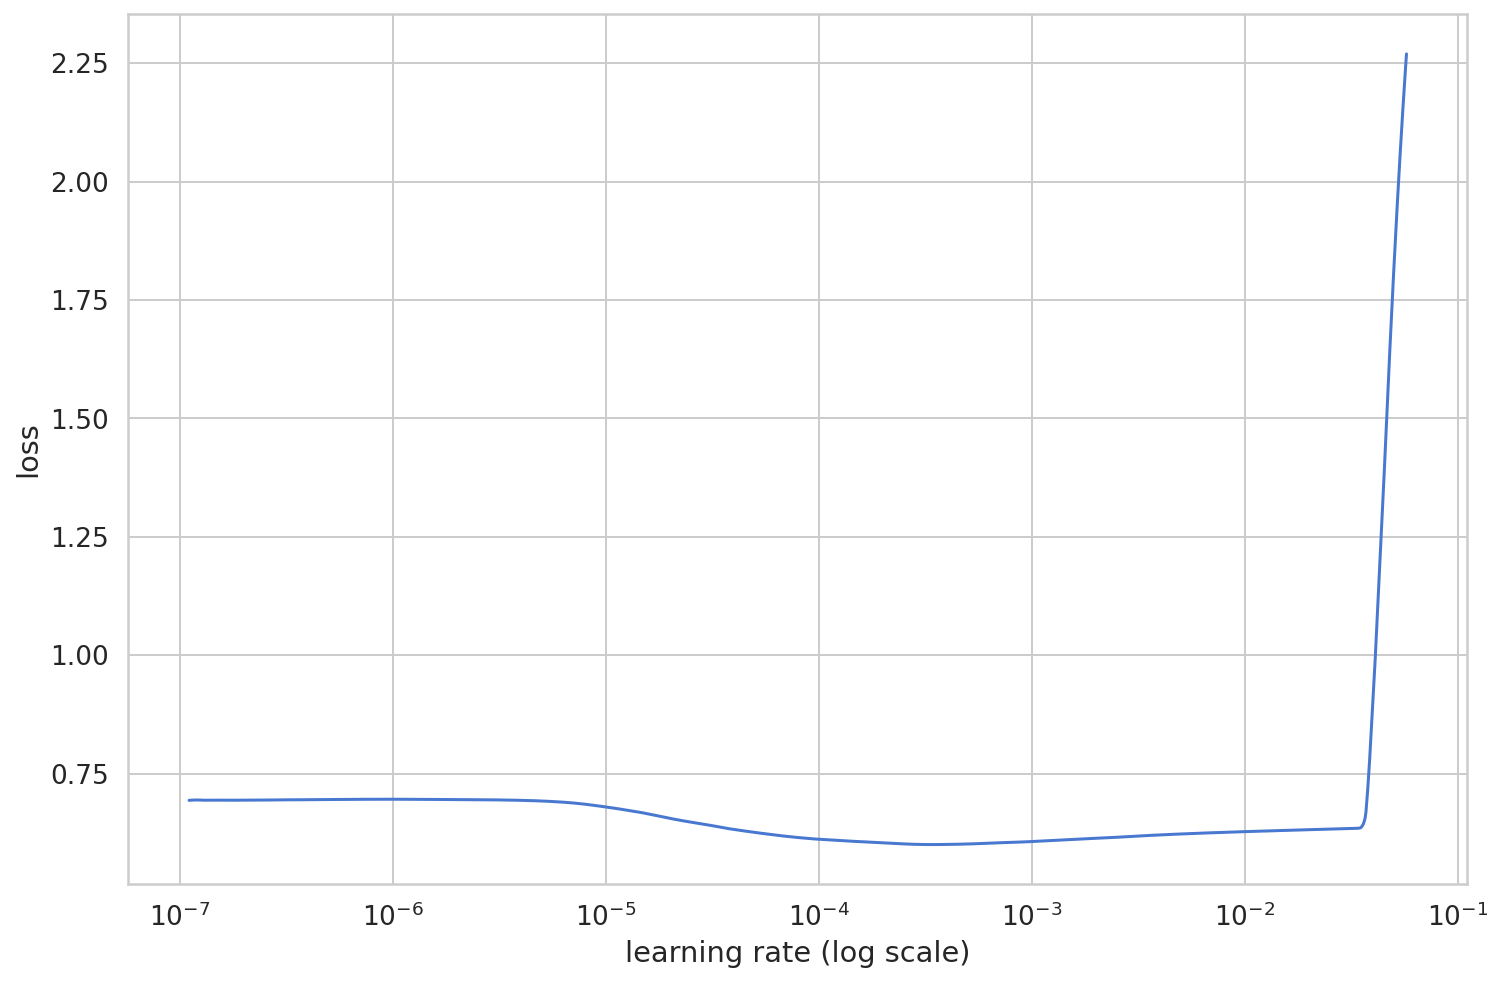
\includegraphics[width=1\textwidth]{images/output_97_0.png}
\caption{Ktrain learner plot}
\label{fig:fig_29}
\end{figure}
\FloatBarrier

\paragraph{fit\_onecycle}
The fit\_onecycle method is better in speed and accuracy as just the fit method.
The fit\_onecycle is an implementation of Leslie Smith’s 1cycle policy \cite{smith_disciplined_2018}.
By using the function:
    \begin{tcolorbox}[breakable, size=fbox, boxrule=1pt, pad at break*=1mm,colback=cellbackground, colframe=cellborder]
\begin{Verbatim}[commandchars=\\\{\},fontsize=\footnotesize]
\PY{n}{learner}\PY{o}{.}\PY{n}{fit\PYZus{}onecycle}\PY{p}{(}\PY{n}{lr} \PY{o}{=} \PY{l+m+mf}{3e\PYZhy{}5}\PY{p}{,} \PY{n}{epochs}\PY{o}{=}\PY{l+m+mi}{4}\PY{p}{)}
\end{Verbatim}
\end{tcolorbox}

 \begin{Verbatim}[commandchars=\\\{\},fontsize=\footnotesize]
begin training using onecycle policy with max lr of 3e-05{\ldots}
Epoch 1/4
23270/23270 [==============================] - 2593s 110ms/step - loss: 0.3926 -
accuracy: 0.8214 - val\_loss: 0.3282 - val\_accuracy: 0.8553
Epoch 2/4
23270/23270 [==============================] - 2587s 110ms/step - loss: 0.3142 -
accuracy: 0.8632 - val\_loss: 0.3245 - val\_accuracy: 0.8584
Epoch 3/4
23270/23270 [==============================] - 2587s 110ms/step - loss: 0.2734 -
accuracy: 0.8844 - val\_loss: 0.3210 - val\_accuracy: 0.8600
Epoch 4/4
23270/23270 [==============================] - 2588s 110ms/step - loss: 0.1708 -
accuracy: 0.9318 - val\_loss: 0.4025 - val\_accuracy: 0.8537
    \end{Verbatim}
At the 4th epoch I have about 85\% accuracy.

\paragraph{validate}
Using the:
    \begin{tcolorbox}[breakable, size=fbox, boxrule=1pt, pad at break*=1mm,colback=cellbackground, colframe=cellborder]
\begin{Verbatim}[commandchars=\\\{\},fontsize=\footnotesize]
\PY{n}{learner}\PY{o}{.}\PY{n}{validate}\PY{p}{(}\PY{p}{)}
\end{Verbatim}
\end{tcolorbox}method I can create a confusion matrix on the newly trained data in order to get a more detailed picture:
    \begin{Verbatim}[commandchars=\\\{\},fontsize=\footnotesize]
              precision    recall  f1-score   support

           0       0.85      0.86      0.85     17380
           1       0.86      0.85      0.85     17525

    accuracy                           0.85     34905
   macro avg       0.85      0.85      0.85     34905
weighted avg       0.85      0.85      0.85     34905

    \end{Verbatim}
            \begin{tcolorbox}[breakable, size=fbox, boxrule=.5pt, pad at break*=1mm, opacityfill=0]
\begin{Verbatim}[commandchars=\\\{\},fontsize=\footnotesize]
array([[14883,  2497],
       [ 2610, 14915]])
\end{Verbatim}
\end{tcolorbox}
        

\paragraph{autofit}
Not satisfied with this result I tried whit autofit \cite{noauthor_amaiyaktrainautofit_nodate}.
Next, I called the function as below:
    \begin{tcolorbox}[breakable, size=fbox, boxrule=1pt, pad at break*=1mm,colback=cellbackground, colframe=cellborder]
\begin{Verbatim}[commandchars=\\\{\},fontsize=\footnotesize]
\PY{n}{learner}\PY{o}{.}\PY{n}{autofit}\PY{p}{(}\PY{l+m+mf}{3e\PYZhy{}5}\PY{p}{,} \PY{n}{reduce\PYZus{}on\PYZus{}plateau}\PY{o}{=}\PY{l+m+mi}{3}\PY{p}{,} \PY{n}{checkpoint\PYZus{}folder}\PY{o}{=}\PY{l+s+s1}{\PYZsq{}}\PY{l+s+s1}{./checkpoint/}\PY{l+s+s1}{\PYZsq{}}\PY{p}{)}
\end{Verbatim}
\end{tcolorbox}

 \begin{Verbatim}[commandchars=\\\{\},fontsize=\footnotesize]
early\_stopping automatically enabled at patience=5

begin training using triangular learning rate policy with max lr of 3e-05{\ldots}
Epoch 1/1024
23270/23270 [==============================] - 2593s 110ms/step - loss: 0.1924 -
accuracy: 0.9222 - val\_loss: 0.4034 - val\_accuracy: 0.8520
\dots
Epoch 6/1024
23270/23270 [==============================] - 2588s 110ms/step - loss: 0.0412 -
accuracy: 0.9842 - val\_loss: 0.7817 - val\_accuracy: 0.8460
Restoring model weights from the end of the best epoch.
Epoch 00006: early stopping
Weights from best epoch have been loaded into model.
    \end{Verbatim}

\subsubsection{Discuss the limitations} 
As can be seen from the autofit code, also in this case I do not exceed 85\% accuracy on validation data, having also here a problem of overfitting.

I then wanted to see what the data was where I had the most loss, this is possible due to:learner.view\_top\_losses(n=1),\\
with the result: id:11764 | loss:8.19 | true:1 | pred:0).\\
\\
At this point I saved the model and weights so that I would have a starting point for next time.\\
I made a list of improvements I want to make in the next test.\\
In text\_from\_df function:
\begin{itemize}
    \item label\_columns = must be a list, so I have to modify this argument,
    \item label\_columns = I can try wiht two different target columns positive and negative (so edit the dataframe),
    \item val\_df = none, so the 10\% of documents in training dataframe will be used for testing/validation,
    \item maxlen = from 400 to 500,
    \item random\_state = none, to have train/test split random.
\end{itemize}

I want also to use the Interactive Training \cite{jupyter_1204}.

\subsubsection{Lesson learned}
The most important of these improvements is missing, which is the work on the dataset.
In fact, the 85\% accuracy is due to the fact of how I made the split between positive and negative reviews.


\subsection{Third model: Ktrain - Hotel dataset optimized}
The idea for this phase is to reduce the review window, focusing only on the actual negative reviews and the very positive reviews.
The continuation for this phase is as follows:
\begin{itemize}
    \item resume the original dataset,
    \item take only the best and worst reviews, based on the "Review\_Score" column,
    \item make a resample, so that you have the two categories in equal measure,
    \item and the other improvements described in the previous chapter.
\end{itemize}

\subsubsection{Improvements}
After making the improvements described above, I was able to create a model with an accuracy for the English language of 96\%.

\subsection{Fourth model: Automatic Ktrain - Filmstarts dataset}
\label{chap:model filmstars auto}
In Switzerland the greater part of the newspaper articles are in German language, and for this reason the models that I have trained up to this moment are not suitable to the task that they must execute, therefore I have created a new model for the German language on the base of the previous models.
Fortunately, the basis I have for creating the model is correct, what I had to do is look for a suitable dataset.
For this assignment I chose a dataset on German movies, although it was difficult to find.
For training I did exactly the same as for the previous models, so I have:
\begin{itemize}
    \item clean the dataset,
    \item I have taken in consideration for the model only the more opportune data,
    \item trained model thanks to Ktrain.
\end{itemize}

\subsubsection{Major changes}
For this model I used as in the previous Ktrain, with these modifications:
\begin{itemize}
    \item BERT instead of distilBERT for greater accuracy with the German language,
    \item automatic model,
\end{itemize}
arriving at an accuracy of 90\%.

\subsubsection{Discuss the limitations} 
Now that I have a trained model I tried testing with a file. The file consists of 30 news articles in German.

To do this test I manually labelled each item positive/negative creating a ground true and then compared it to what the model predicted.

What I saw was that the model correctly predicted most articles, with a few issues where the article was a fact or neutral, but this is normal since I only trained for positive and negative.
Unfortunately, despite the model arrives at a good percentage (90\%) I noticed that some articles where it is clearly negative were predicted positive. 

At this point I thought the problem was with the dataset and the model so here are the improvements I want to make in the next one:
\begin{itemize}
    \item take in consideration only 0 and 5 from the dataset,
    \item modify ktrain.
\end{itemize}